\begin{figure*}[ht]
\begin{minipage}{.7\textwidth}
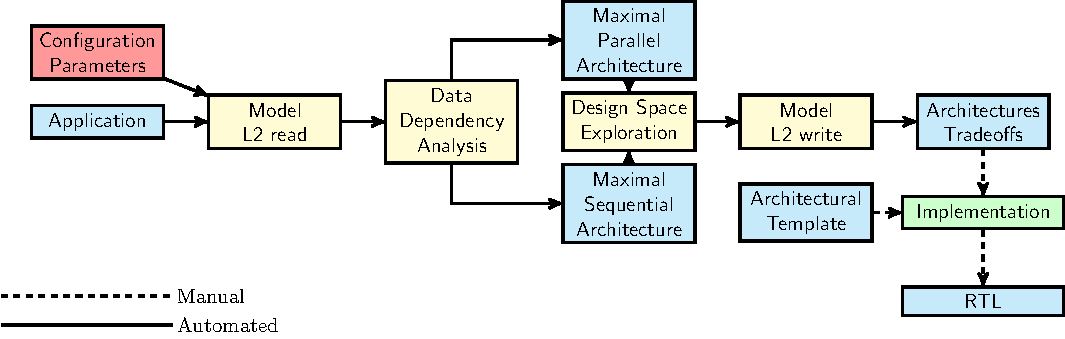
\includegraphics[width=\textwidth,left]{images/framework.pdf}
  \caption{\small \frameworkname~Framework.}{}
  \label{fig:framework}
\end{minipage}%
\begin{minipage}{.3\textwidth}
    \centering
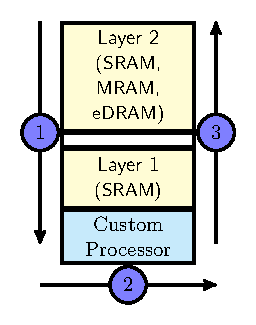
\includegraphics[width=.5\textwidth]{images/architecture.pdf}
\caption{\small The system under analysis. 
    }
\label{fig:system}
\end{minipage}
\end{figure*}
\section{The \frameworkname~framework}
\label{sec:framework}
The framework presented in this work allows the user to \textbf{customize} the different building blocks to be used in the co-design of the custom processor and memory system, \textbf{explore} custom architectures automatically generated for a given application, and \textbf{estimate} area, power and latency of each one of the architectures. The \frameworkname~framework, illustrated in Figure~\ref{fig:framework} takes two inputs, the \textit{Configuration Parameters} - described in Section~\ref{ssec:conf_param} - and an \textit{Application} - detailed in Section~\ref{ssec:app}, and automatically generates set of hardware architectures, behaviorally equivalent to the input application. Additionally, the analysis of area, power and latency of these architectures is automatically produced. The generated hardware architectures can be used to generate an RTL implementation using the \textit{architectural templates} described in Section~\ref{sec:arch_template}.
The rest of this section provides a detailed analysis of the design and implementation of \frameworkname.
 

\subsection{Model of Execution}
\label{ssec:system_under_analysis}
The system architecture we assume in this work is composed of two levels of memory and a custom processor, as shown in Figure~\ref{fig:system}. Level 1 memory (L1M)\footnotemark, the first memory lavel, and the smaller one in size, uses SRAM as it needs to be physically close to the processor for faster access. The second level - Level 2 memory (L2M)\footnotemark[\value{footnote}] - larger in size and can be implemented using any memory technology (on-chip or off-chip), even with with different access latency for read and write operations. Note that the processor and L1M run at a different clock speed than the L2M. 
\footnotetext{These memories are not caches and we do not use cache policies because we schedule data movements at design time. To clarify this we refer to Levels of memory instead of Layers and we abbreviate using L1M and L2M instead of L1 and L2.}
We assume a model of execution, following the three steps illustrated in Figure~\ref{fig:system}. Initially, all of the required input data for the application are available at the L2M. Next, the input data is transferred to the processor using L1M as intermediate storage (step 1), the data is processed and the results are temporarily stored in L1M (step 2), and finally the data from L1M is transferred back to L2M (step 3). Note that our model of execution performs the steps in a pipelined manner, hence only part of the data will be stored in L1M at any given time. 

%Taking advantage of the possibility to produce stacked chip having levels produced using different manufacturing technologies we are able to explore different memory implementations at the L2 of the memory architecture.

%\begin{figure}[tb] 
%\centering
%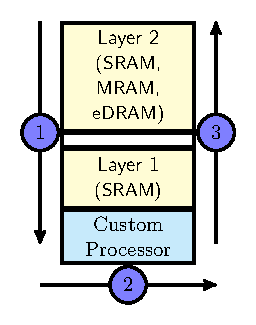
\includegraphics[width=0.25\columnwidth]{images/architecture.pdf}
%\caption{\small The system under analysis. Composed by two levels of memory, the memory at layer two can use various technologies while the memory at layer one uses only SRAM technology.}
%\label{fig:system}
%\end{figure}

\subsection{L2 Memory Model}
\label{ssec:layer2_model}
Since the L2M has higher access latency, we model them assuming the data is accessed in larger bursts.
%Figure~\ref{fig:l2model}  shows a representation of such access. 
A read or write burst access to the L2M is controlled by a Direct Memory Access (DMA) controller, with the starting address and size of the burst given as input to the DMA. After an initial \textit{setup latency}, the accessed elements are transferred in sequence from the start address to the end address, from L1M to L2M in case of a write, and from L2M to L1M in case of a read.

\subsection{Application}
\label{ssec:app}
The framework performs exact data dependency analysis on the input application, thus requiring that the behavior of the application is completely specified at compile-time, and independent from the input data. The input application language that our framework currently supports is C/C++, however the framework uses the LLVM Intermediate Representation~\cite{llvm}, so it can be easily extended to support other languages as well.
%\begin{lstlisting}[language=C, caption={Example of input application, C implementation of a matrix vector multiplication.}, label={lst:matrixvec}]
%void matrix_vec_kernel(int *A,int *B, int *C){
%    int sum;
%    for(int i=0;i<DIM2;i++){
%        sum=0;
%        for(int j=0;j<DIM1;j++){
%            sum+=A[i*DIM1+j]*B[j];
%        }
%        C[i]=sum;
%    }
%}
%\end{lstlisting}

\subsection{Configuration Parameters}
\label{ssec:conf_param}
The second input to the framework is a configuration file for the different building blocks to be used in for hardware architecture realization. Through this file, the user can specify: different compute units (e.g. multipliers, adders), process technology to be used (e.g. 16nm, 28nm), the clock frequency of processor and L1M, and the clock frequency L2M. Moreover, the user can specify the datawidth used by the compute units, L1M and L2M. 
Information to model the L2M burst accesses is also specified in this file: the setup latency for write/read accesses, the type of L2M to be used (e.g. MRAM, SRAM) and the size of the L2M. The different parameters in the configuration file are then used to access a database containing estimates (obtained by synthesis or from specs) of area usage, static and dynamic power, and latency of each of the building blocks.

%\begin{lstlisting}[language=json, caption={Example of input configuration file}, label={lst:conf_file}]
%{ 
%   "resource_database": { 
%	"technology": 16, 
%	"clock_frequency": 1000, 
%	"bitwidth_adder": 128, 
%	"bitwidth_multiplier": 64, 
%	"bitwidth_register_file": 128, 
%	"type_l2": "tt1v1v85c", 
%	"technology_l2": 16, 
%	"clock_l2": 800, 
%	"bitwidth_l2": 32, 
%	"depth_l2":2048, 
%	"setup_write_latency_l2":2, 
%	"setup_read_latency_l2":2 
%   } 
%}
%
%\end{lstlisting}

\subsection{L2 Memory Read}
\label{ssec:l2_read_model}
The first operation performed by the framework is to compute the transfer time of the application's input data from L2M to L1M. An address in L2M is given to each input element used by the application; different datastructures are placed in consecutive memory addresses. The entire data transfer is modeled as a single burst read operation to the L2M. The information required to compute the arrival clock time of each input element to the L1M is extracted from the \textit{Configuration Parameters} and performing static analysis on the \textit{Application}.
Using this information, the exact clock at which each input elements arrives in the L1M can be computed as seen in (1),
\begin{equation}
AClk_i = S_r + R_{L2M} * (Add_{L2Mi}+1) * \frac{B_{L1M}}{B_{L2M}} * \frac{Clk_{L1M}}{Clk_{L2M}}
\end{equation}

the symbols are described in Table~\ref{table:equation}.

\begin{table}[]
\begin{tabular}{|l|l|}
\hline
\textbf{Symbol} & \textbf{Definition}                                           \\ \hline
$AClk_i$           & Clock at which element i arrives to the L1M                \\ \hline
$S_r$             & Setup Latency of a L2M burst read                          \\ \hline
$R_{L2M}$       & L2M read latency per read operation, \\ &in L2M clock cycles   \\ \hline
$Add_{L2Mi}$     & Offset of element i from the beginning \\ &of the burst access \\ \hline
$B_{L1M}$        & Data bitwidth of L1M                                       \\ \hline
$B_{L2M}$        & Data bitwidth of L2M                                       \\ \hline
$Clk_{L1M}$      & Clock Frequency of L1M                                     \\ \hline
$Clk_{L2M}$      & Clock Frequency of L2M                                     \\ \hline
$WBL_{L2M}$      & L2M write burst latency                                    \\ \hline
$S_w$             & Setup Latency of a L2M burst write                         \\ \hline
$W_{L2M}$       & L2M write latency per read operation, \\ &in L2M clock cycles  \\ \hline
$O$                 & Total number of output elements                            \\ \hline
\end{tabular}
\caption{Definition of symbols used in the equations}
\label{table:equation}
\end{table}

\subsection{Data Dependency Analysis}
\label{ssec:dda}
The \textit{Data Dependency Analysis (DDA)} module is divided in three stages. First, it extracts the \textit{Data Dependency Graph} (DDG)\cite{isoda1983global} from the application. Then, it schedules the DDG using the As Soon As Possible (ASAP) and As Late As Possible (ALAP) methodologies. Finally, it maps instructions in the DDG to hardware components - or Functional Units (FUs) - using a modified version of the \textit{Interval Partitioning} algorithm~\cite{greedyIntervalPartitioning}.
%This next paragraph might be replaced with a reference

To extract the DDG from an application we use LLVM  and custom transformations. We first convert the input application code to its LLVM Intermediate Representation. We then transform the code into static single assignment (SSA) form and perform full-loop unrolling on all of the application loops. After these transformations, there will be no control flow instructions in the application body, and each variable will be defined only once. It is now possible to follow the definition and use chain of the variables to produce a Data Dependency Graph like the one shown in Figure~\ref{fig:ddg}. 

We further process the obtained DDG, aiming to reduce the length of the path between the input nodes and the output nodes. This additional transformation is important because the length of these paths is equivalent to the number of sequential operations required to obtain the outputs, which in turn determines the latency of the application. Taking advantage of operation associativity (where possible) we can transform a long sequence of operations - like the one highlighted in Figure~\ref{fig:ddg} - into an equivalent shorter tree.
%\begin{figure}[ht]
%\begin{minipage}{.5\textwidth}
%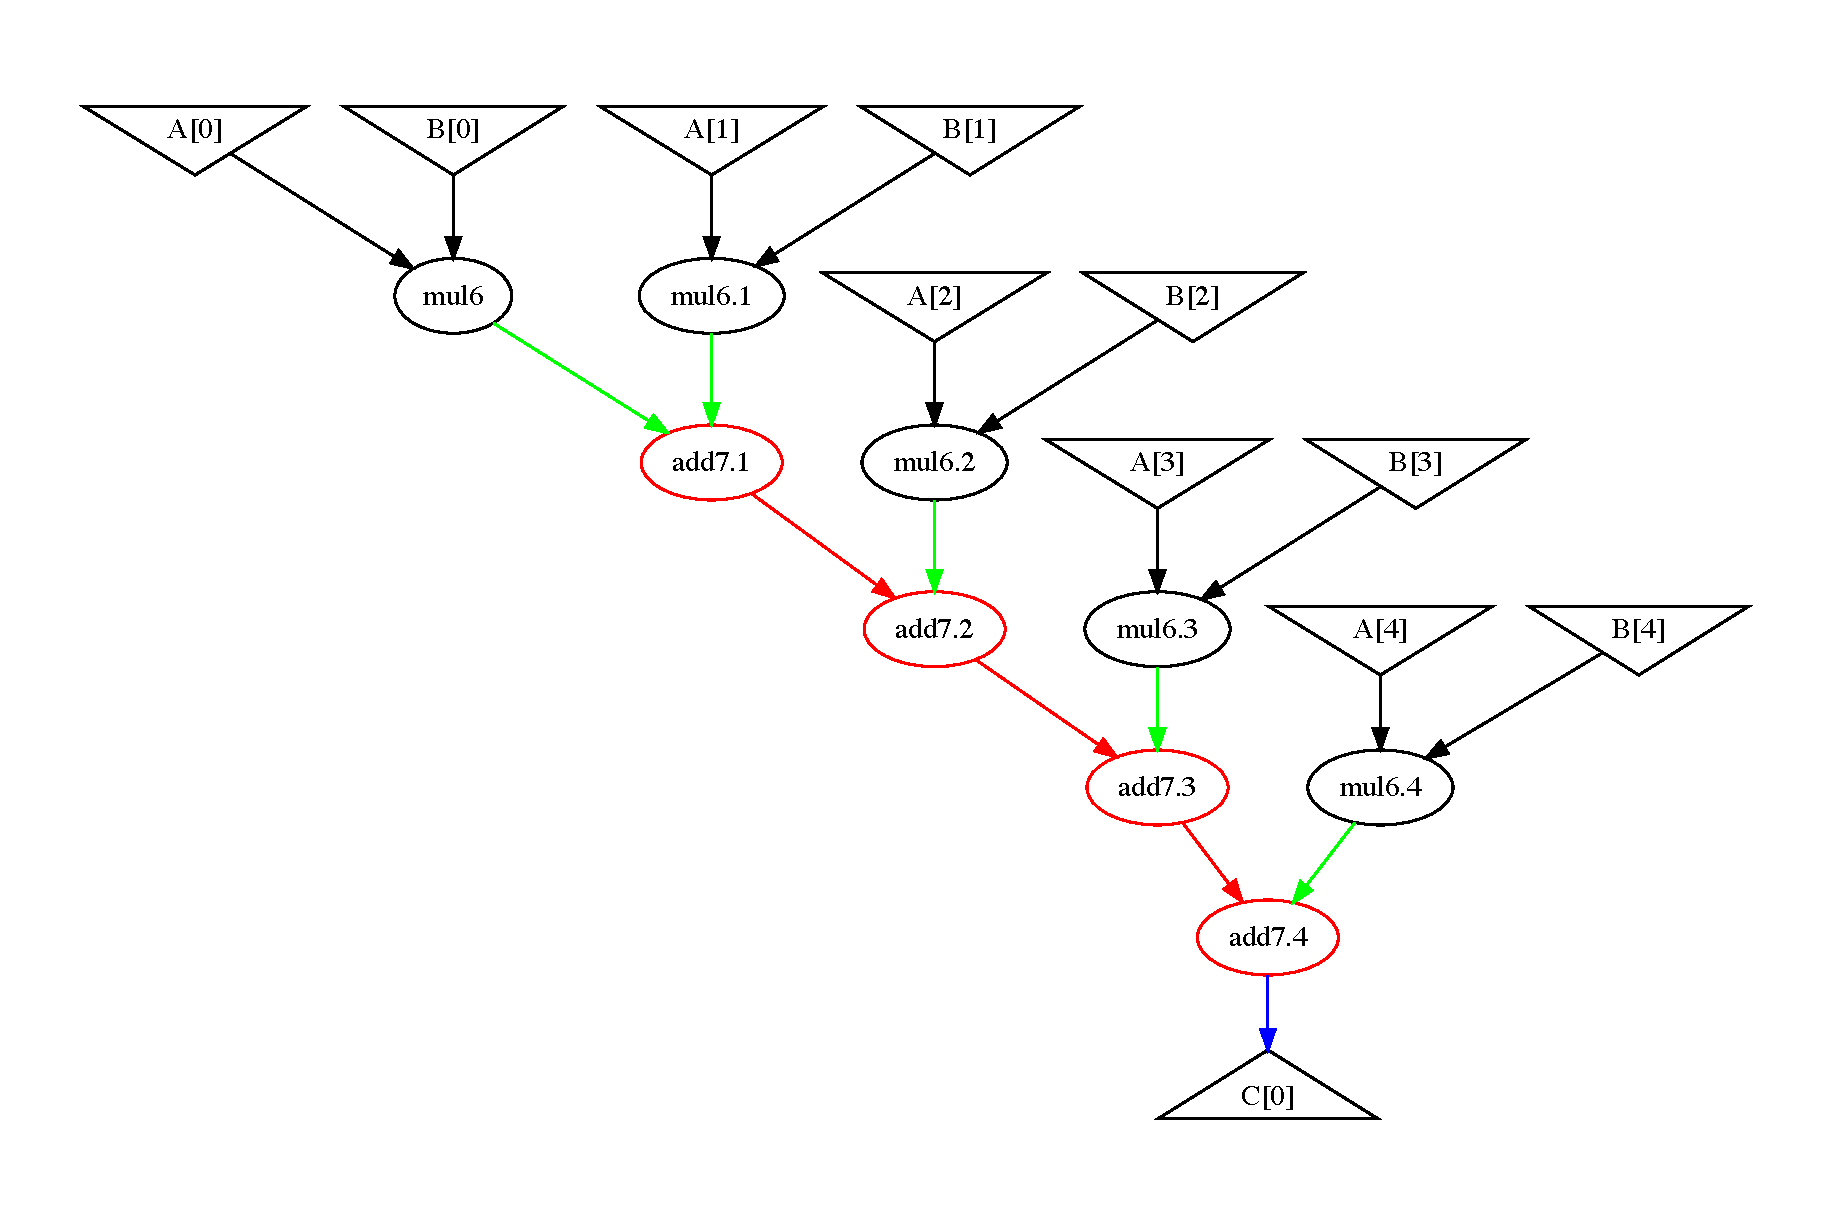
\includegraphics[width=.9\textwidth,left]{images/supernode.pdf}
%  \caption{\small \frameworkname~Framework.}{}
%  \label{fig:framework}
%\end{minipage}%
%\begin{minipage}{.5\textwidth}
%    \centering
%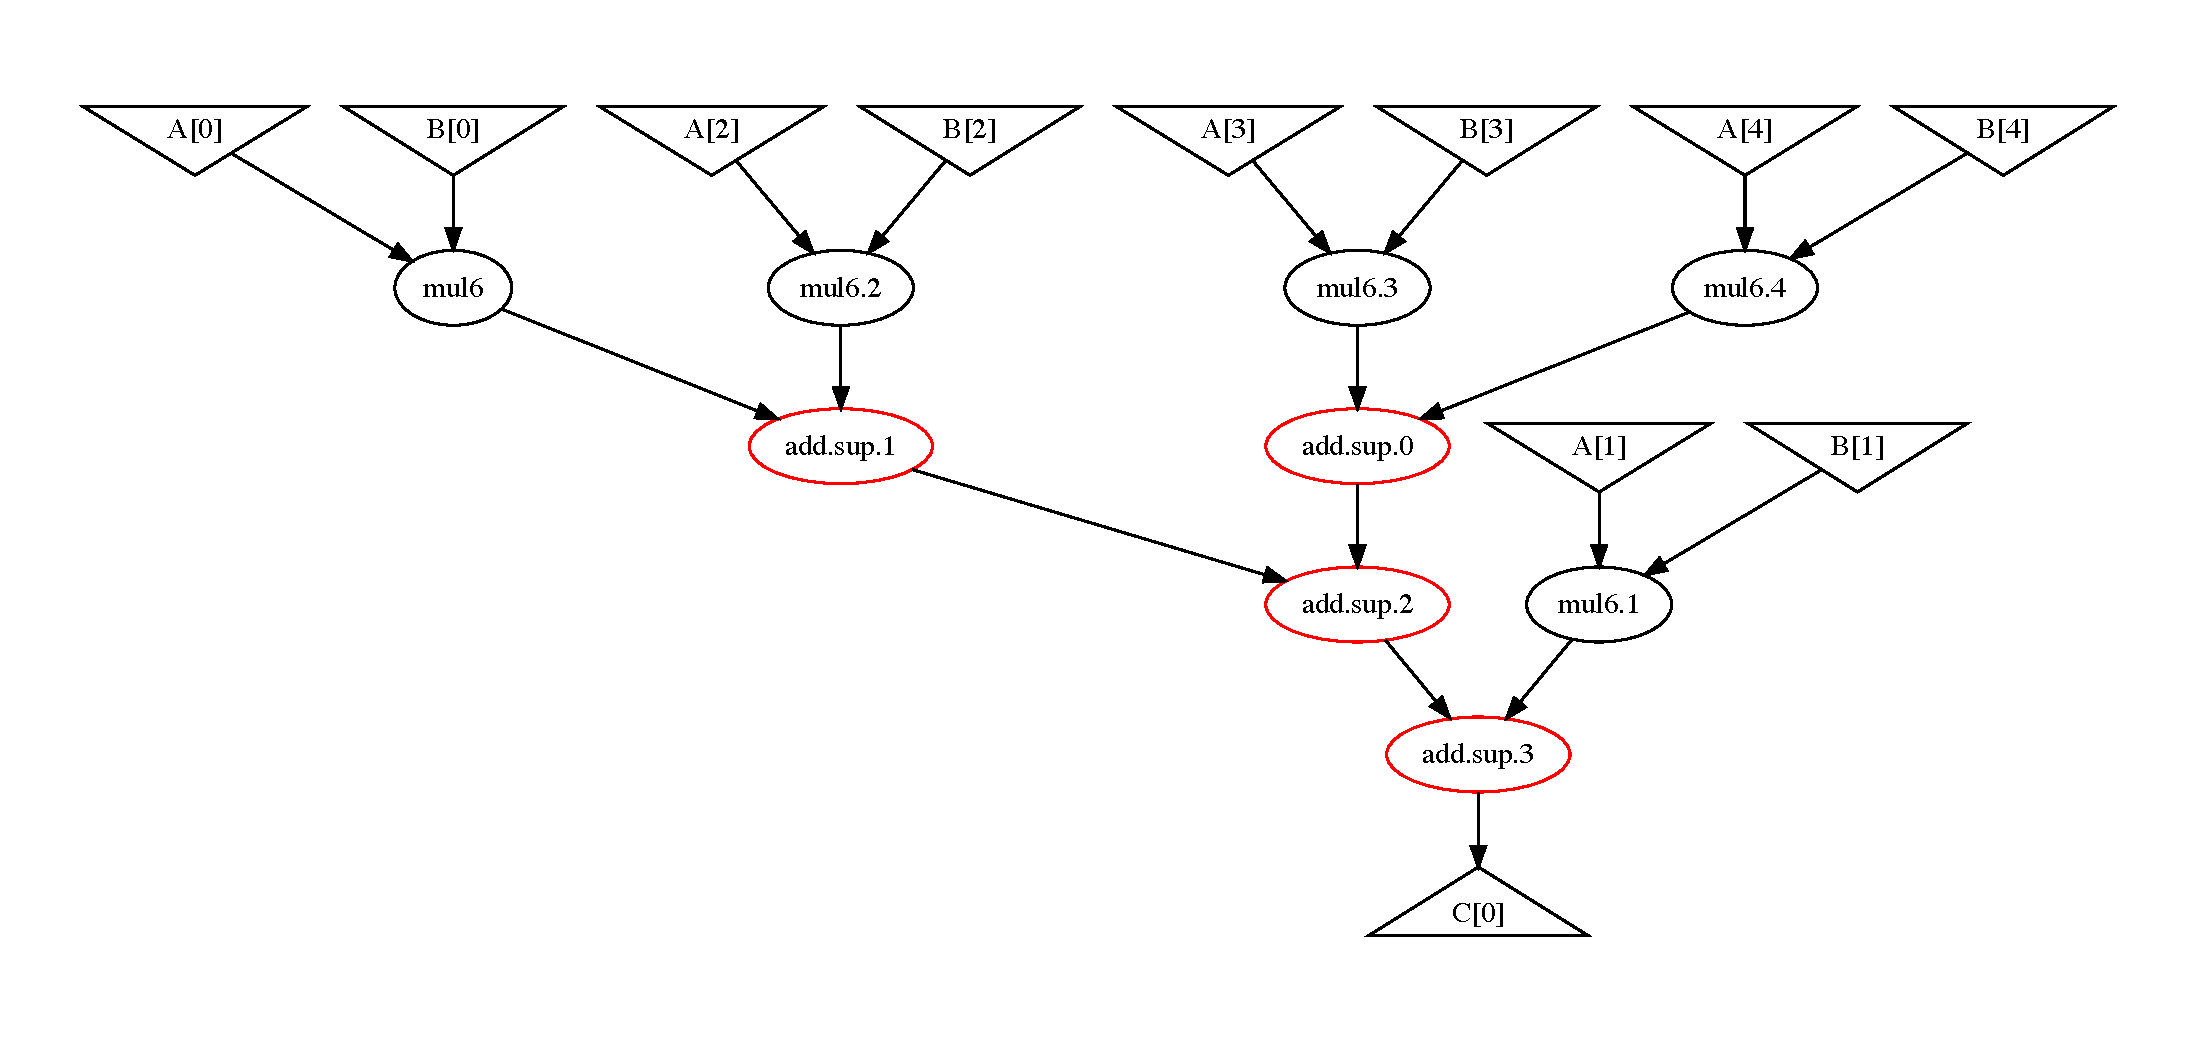
\includegraphics[width=.9\textwidth]{images/supernode_optimized.pdf}
%\caption{\small The system under analysis. 
%    %Composed by two levels of memory, the memory at layer two can use various technologies while the memory at layer one uses only SRAM technology.
%    }
%\label{fig:system}
%\end{minipage}
%\end{figure}

\begin{figure}[tb] 
\centering
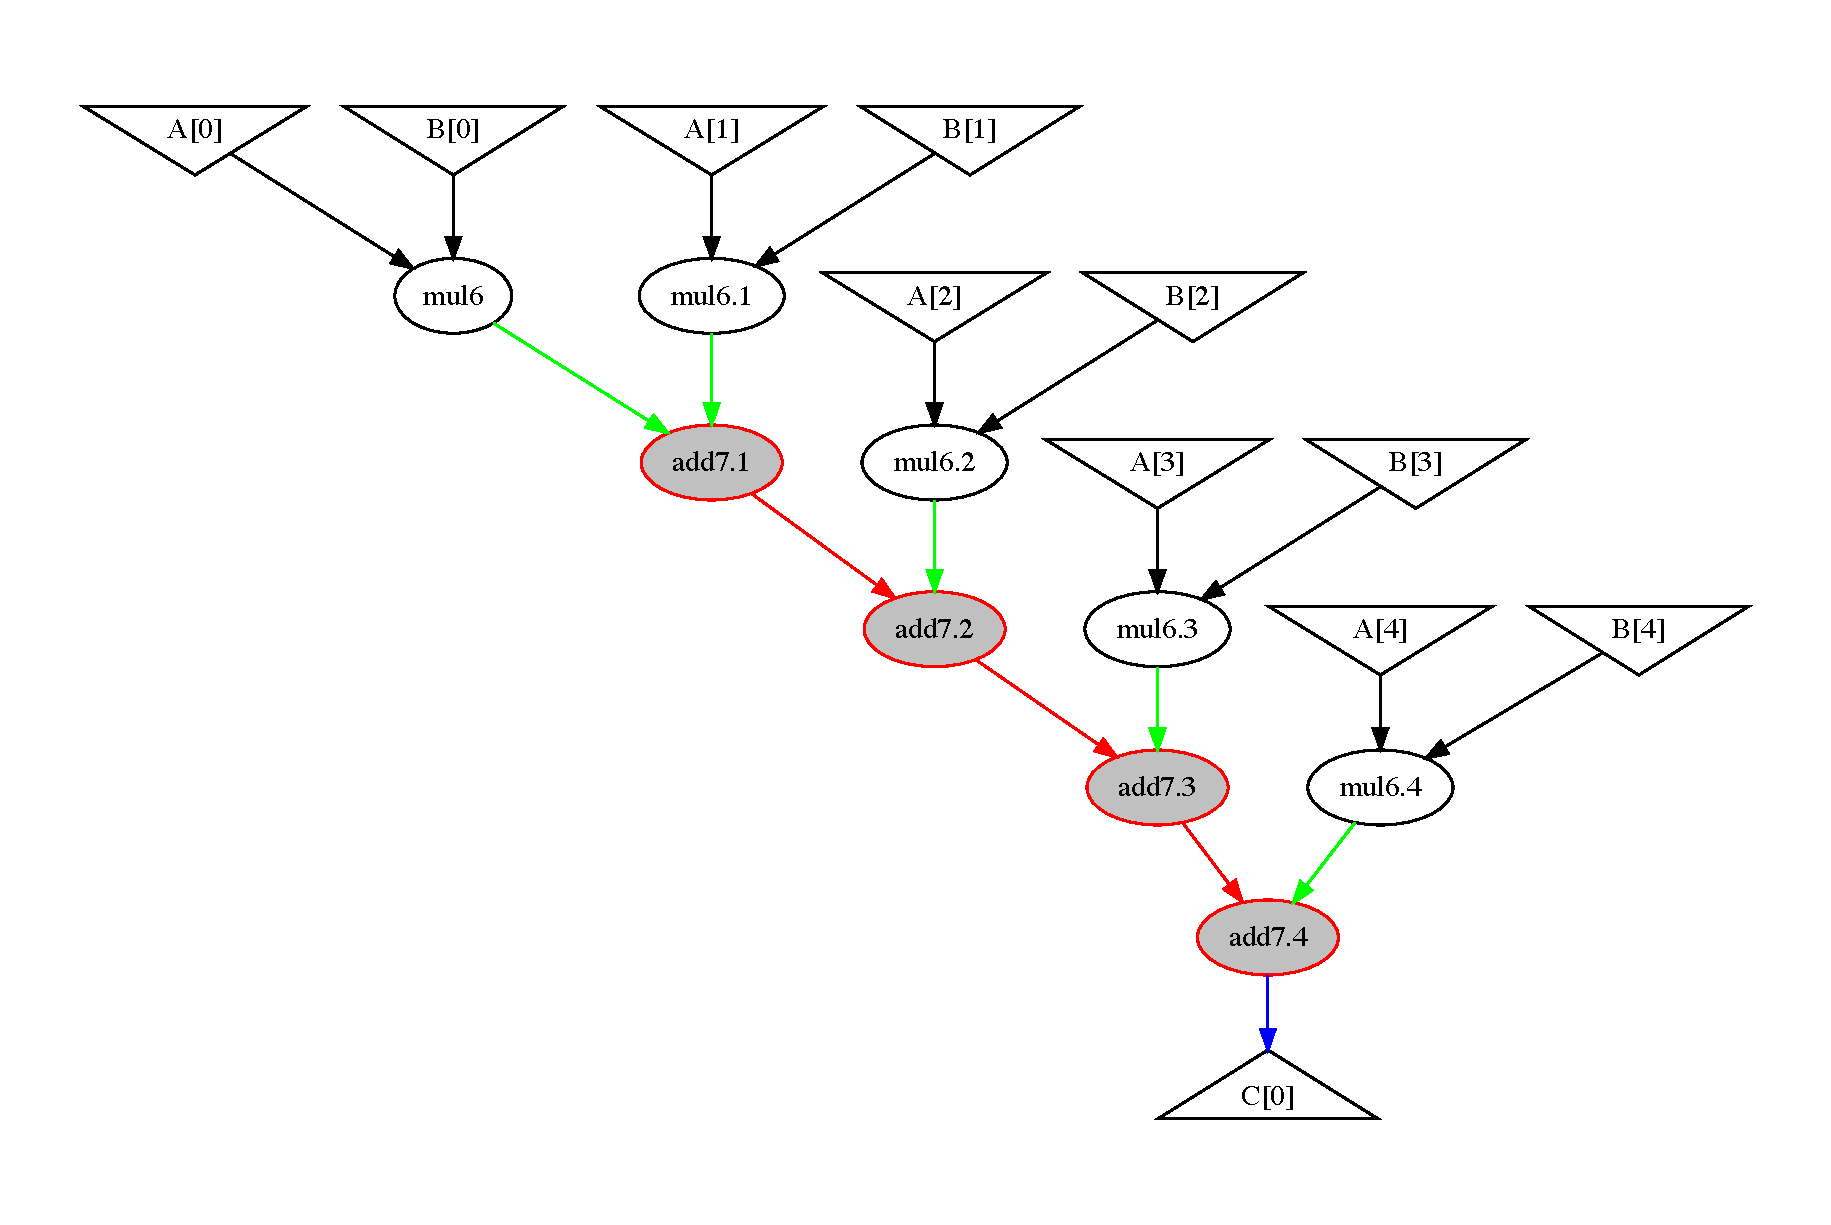
\includegraphics[width=.9\columnwidth,left]{images/supernode_2.pdf}
    \caption{\small Example of Data Dependency Graph. The inverse triangles represent the input data, obtained from the \textit{load} instructions. The ovals describe operations on data, while the triangle at the bottom represents the result, derived from a \textit{store} instruction. Highlighted, a chain of associative operation before it is optimized by the \textit{DDA} module (see \ref{ssec:dda}).}
\label{fig:ddg}
\end{figure}
%This next paragraph might be replaced with a reference, we are interested mainly in the concept of mobility
Once we have the DDG, we apply the ASAP and ALAP scheduling methodologies to the generated DDG. These schedules will associate to each DDG node a clock cycle where the instruction is executed, and \textit{bound} the space of possible architectures by determining the \textit{maximally parallel} architectures. We start by scheduling the input nodes of the DDG using the arrival clock time of their element, computed as explained in Section~\ref{ssec:l2_read_model}, thus taking into account the L2M - L1M transfer time. Next, we determine the minimal latency required to obtain the outputs of the application with the ASAP schedule: starting from the DDG input leafs, each instruction node is scheduled as soon as its dependencies are resolved. 
Once ASAP is completed, we can perform the ALAP scheduling: starting from the output leaf nodes, each node is scheduled as late as possible according to its dependencies. Once ALAP is completed, every node is annotated with an ASAP clock cycle and an ALAP one. The difference between these two clock cycles, called instruction \textit{mobility}, identifies an interval in which the instruction can be scheduled without changing the overall latency of the application.

The final stage of the \textit{Data Dependency Analysis} module - described in Section~\ref{ssec:modified_interval_partitioning} - will allocate the DDG nodes to FUs, leveraging the nodes mobility to minimize the number of FUs of the final hardware architecture. 

\subsection{FU allocation with Modified Interval Partitioning}
\label{ssec:modified_interval_partitioning}
To generate a hardware architecture behaviorally equivalent to the input application and with the latency identified during the ASAP-ALAP scheduling, there are two main requirements: (1) each instruction needs to be computed within its ASAP-ALAP interval, and (2) instructions in the original DDG which are executed by the same FU cannot be scheduled at the same time.
Our Modified Interval Partitioning (MIP) algorithm - based on the original greedy Interval Partitioning algorithm~\cite{greedyIntervalPartitioning} - is designed to generate hardware architectures from a DDG that meet both requirements. The original Interval Partitioning problem addresses the issue of assigning a number of jobs, with known starting and ending time, to the minimum amount of resources, ensuring that the jobs assigned to a resource do not overlap. To use Interval Partitioning for our problem, we consider instructions as jobs and FUs as resources. There are, however, three main differences between our problem and the canonical Interval Partitioning. 
First, the original algorithm considers any job can use any resource, while our architecture requires different FUs for different instructions. We therefore perform interval partitioning several times, once for each instruction type (e.g., four times for the graph in Fig. 4). This ensures a correct allocation of the instruction to FUs performing the same operation. Second, due to \textit{mobility}, instructions do not have a fixed starting time. The MIP takes the mobility of an instruction into account allowing a given instruction to start at any time within its allowed interval. Third, and final difference, is that our instructions are dependent on each other , which is not the case for the jobs in the original interval partitioning. To account for this extra constraint, we ensure that any given instruction (1) is only allocated after its dependencies are allocated, and (2) is scheduled to start after the ending time of its dependencies.
Listing~\ref{lst:modified_interval_partitioning} shows the pseudocode of our modified interval partitioning algorithm. 
\begin{lstlisting}[language=Python, caption={Modified Interval Partitioning Algorithm}, label={lst:modified_interval_partitioning}]
FunctionalUnits=[]
sort i in Instructions by ASAP[i]
for each i in Instructions
	allocated = False
	schedule[i] = ASAP[i]
	for d in dep(i)
		end_time_d = schedule[d] + latency(d)
		schedule[i] = max(schedule[i],end_time_d)
	for each fu in FunctionalUnits 
		if type(fu) ==  type(i)
			if ALAP[i] >=  next_free_slot[fu]
				fu += [i]
				schedule[i] = max(schedule[i],
					next_free_slot[fu])
				next_free_slot[fu] = schedule[i] + 
					latency(i)
				allocated = True
	if not allocated
		create new Functional Unit fu
		type(fu) = type(i)
		fu += [i]
		next_free_slot[fu] = schedule[i] + latency(i)
		FunctionalUnits += [fu]

\end{lstlisting}
We assume that ASAP and ALAP schedules have been previously performed, hence we can have two datastructures that return the ASAP and ALAP schedules for a given instruction i - i.e. ASAP[i] and ALAP[i]. Instructions is an ordered list of instructions initialized with the instructions of the input application. A Functional Unit is represented as a set containing the instructions that have been allocated to it, and FunctionalUnits is a set containing the Functional Units of the resulting architecture which is initialized as an empty set. The functions latency and dep take an instruction i as input and return respectively the latency of i and a list of instructions i depends on. The function type
takes as input a Functional Unit or an Instruction and returns the type of operation performed.
The MIP algorithms returns the FunctionalUnits and schedule datastructure. FunctionalUnits contains a set of Functional Units which define the generated architecture, each Functional Unit is a set that contains the instructions to be executed. The schedule datastructure will contain the clock at which each instruction of the input application has to be executed.

\subsection{Most Parallel and Most Sequential Architectures}
The result of the \textit{DDA} module is the \textbf{Most Parallel Architecture (MostPar)}. This architecture takes full advantage of the parallelism of the application and performs the computation with the minimum latency. However, the MostPar uses the maximum number of FUs - in the worst case scenario equivalent to the number of instructions in the application - and it will hence have the worst area.
At the other end of the spectrum of architectures we can imagine the \textbf{MostSeq (MostSeq)}, where no parallelism is used and the instruction are scheduled sequentially respecting their dependencies. This architecture will have the worst possible latency, however the minimal impact in area - using only one FU per operation type.
Probably none of these two architectures will be of direct interest for the user as they represent two extreme cases. The architecture that are most likely to be interesting are the ones between the \textbf{MostPar} and \textbf{MostSeq} that offer tradeoffs between power, latency and area. Section~\ref{ssec:dse} describes how these intermediate architectures can be procedurally generated.

\subsection{Design Space Exploration}
\label{ssec:dse}
The \textit{Design Space Exploration} \frameworkname~module procedurally generates hardware architectures, behaviorally equivalent to the input application, which exhibit area, latency and power tradeoffs. 
Our DSE is an iterative process which outputs, at the end of each iteration, a different hardware architecture. 
The iterative process start its sweep from the \textbf{MostPar}, and ends when the \textbf{MostSeq} is generated. 
An iteration consists of three steps. First, the instructions corresponding to output leaf nodes in the DDG are selected. The ALAP schedule of these iterations is increased by 1, and the ALAP scheduling of the rest of the nodes in the DDG is updated accordingly. Consequently, the mobility of each instruction node is increased by one. Finally, the MIP is ran again, using the new ALAP schedule. Due to the increased mobility of each instruction the generated architecture is likely to use less FUs.
The process stops as soon as one iteration generates the \textbf{MostSeq}, which can be recognized because it contains only one FU per operation type.

There are two side benefits of our DSE approach. First, the user can tune the granularity of the exploration: by increasing the ALAP "slack" beyond 1, the exploration speeds-up, but less architectures are generated. Second, the DSE process can be easily parallelised, because its iterations are independent of each other.


\subsection{L2 Memory Write}
The schedule produced by MIP includes the L2M-L1M transfer, and the computation; it does not include the L1M-L2M transfer. However, due to MIP, we do know the clock cycle at which computation ends (phase 2 in Figure~\ref{fig:system}) and the last data item is written in L1M. The L1M-L2M transfer can start immediately after the last output is generated.
The latency of the L1M-L2M transfer is calculated using (2),
\begin{equation}
    WBL_{L2M} = S_w + W_{L2M} * O * \frac{B_{L2M}}{B_{L1M}} * \frac{Clk_{L1M}}{Clk_{L2M}}
\end{equation}
where the symbols have been defined in Table~\ref{table:equation}

\subsection{Architecture Tradeoffs}
%In section~\ref{
For a given input application and a given configuration (see Figure \ref{fig:framework} \frameworkname~outputs a set of hardware architectures having different area and latency tradeoffs. Figure~\ref{fig:tradeoffs} shows three of the architectures generated during the DSE. Each box represents a FU. The FUs generated from load and store instructions become separate L1M banks. The remaining FUs are obtained from processing instructions. We allow the architectures to have cycles because the circuit is synchronousi, and every instruction has been carefully scheduled. A self-loop in a FU identifies data reuse (see Section~\ref{sec:arch_template} for implementation details).
\begin{figure}[ht]
\centering
\begin{subfigure}{.4\columnwidth}
  \centering
  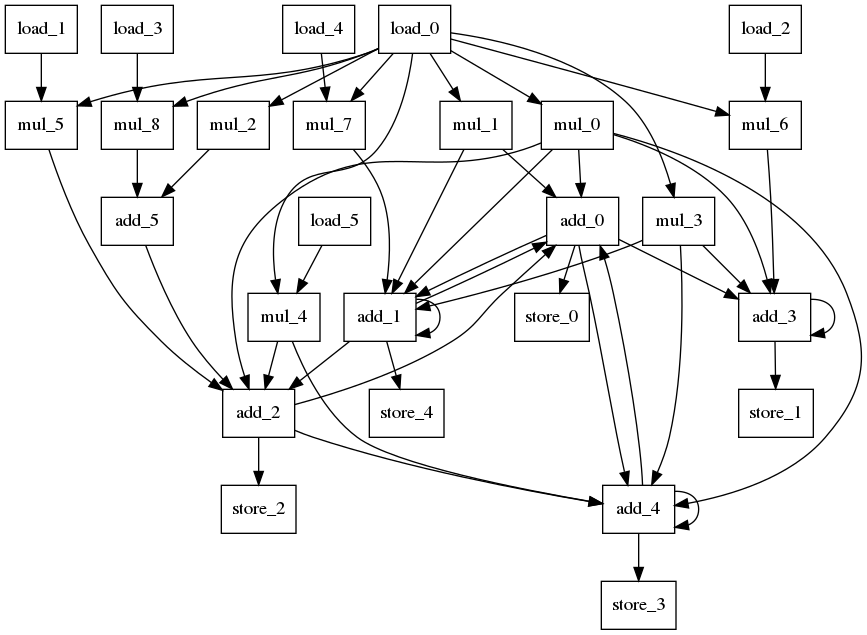
\includegraphics[width=\textwidth]{images/Architecture_latency_146_schematic.png}
  \caption{}
  \label{fig:max_par_arch}
\end{subfigure}%
\begin{subfigure}{.3\columnwidth}
  \centering
  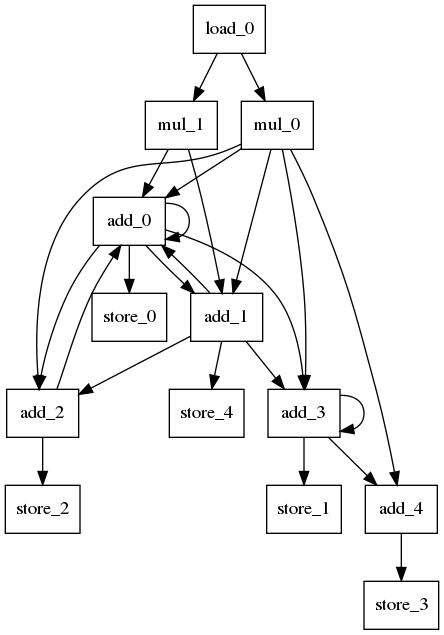
\includegraphics[width=\textwidth]{images/Architecture_latency_166_schematic.png}
  \caption{}
  \label{fig:inter_arch}
\end{subfigure}
\begin{subfigure}{.2\columnwidth}
  \centering
  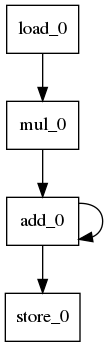
\includegraphics[width=0.5\textwidth]{images/Architecture_latency_188_schematic.png}
  \caption{}
  \label{fig:most_seq_arch}
\end{subfigure}
    \caption{\small Example of architectures generated from a matrix vector multiply application of size 5x5. The MostPar (a), an intermediate architecture (b) and the MostSeq (c).}
\label{fig:tradeoffs}
\end{figure}

%\begin{figure}
%
%\begin{minipage}{.5\linewidth}
%\centering
%\subfloat[]{\label{main:a}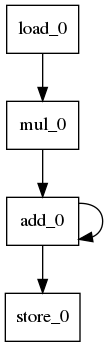
\includegraphics[scale=.2]{images/Architecture_latency_188_schematic.png}}
%\end{minipage}%
%\begin{minipage}{.5\linewidth}
%\centering
%\subfloat[]{\label{main:b}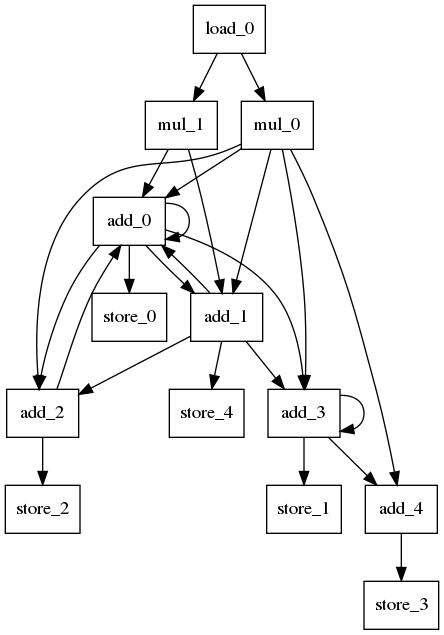
\includegraphics[scale=.2]{images/Architecture_latency_166_schematic.png}}
%\end{minipage}\par\medskip
%\centering
%\subfloat[]{\label{main:c}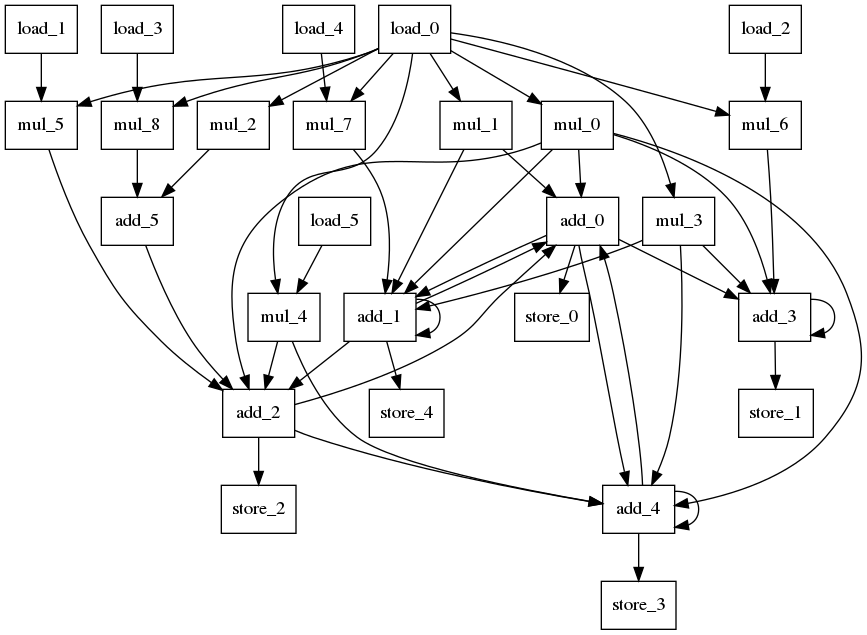
\includegraphics[scale=.10]{images/Architecture_latency_146_schematic.png}}
%
%\caption{my fig}
%\label{fig:main}
%\end{figure}
